\subsubsection{UC26 - Garage veicolo}
\begin{figure}[h]
	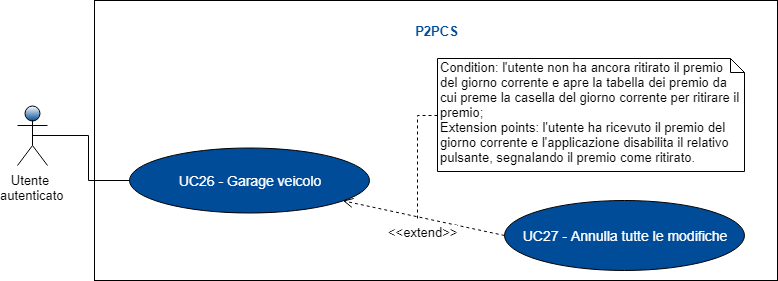
\includegraphics[width=9cm]{res/images/UC26Garage.png}
	\centering
	\caption{UC26 - Garage veicolo}
\end{figure}
\begin{itemize}
	\item \textbf{Attori Primari}: utente autenticato;
	\item \textbf{Descrizione}: agli utenti autenticati è reso disponibile un Minigioco composto da un garage dove si possono fare modifiche ad un'auto base di partenza tramite rewards ottenuti da sblocchi di obbiettivi e al superamento di livelli d'esperienza personale grazie ad un'utilizzo dell'applicazione in modo continuo. \\ Ogni pezzo di ogni tipo di modifica, installato sul veicolo, visualizza in punteggio le seguenti informazioni:
	\begin{itemize}
		\item velocità;
		\item accelerazione;
		\item peso;
		\item maneggevolezza.
	\end{itemize}
	punteggi che poi verranno sommati e attribuiti come statistiche al veicolo e visualizzate nella schermata principale dell'auto; 
	\item \textbf{Scenario principale}: l'utente accede al Minigioco e visualizza un'auto base con la possibilità di modificarla attraverso due categorie:
	\begin{itemize}
		\item Prestazione [UC26.1];
		\item Estetica [UC26.2];
	\end{itemize}
	e successivamente se le modifiche apportate vanno bene all'utente, può installarle e confermarle;
	\item \textbf{Estensioni}:
	\begin{itemize}
		\item annulla tutte le modifiche [UC27].
	\end{itemize}
	\item \textbf{Precondizione}: l'utente autenticato ha selezionato la voce \textit{Garage} dal menu dell'applicazione;
	\item \textbf{Post-condizione}: l'utente autenticato ha visualizzato la sua auto e installato le modifiche se attuate. 
\end{itemize}
\subsubsection{UC26.1 - Prestazione}
\begin{figure}[h]
	%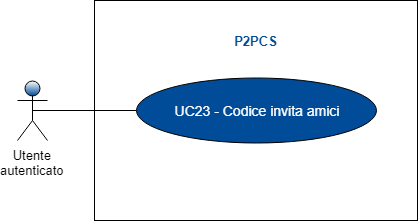
\includegraphics[width=9cm]{res/images/UC23Codiceamico.png}
	\centering
	\caption{UC26.1 - Prestazione}
\end{figure}
\begin{itemize}
	\item \textbf{Attori Primari}: utente autenticato;
	\item \textbf{Descrizione}: l'utente accede alla categorie di modifiche sulla prestazione per la propria auto. Avrà a disposizione un tot di pezzi per ogni singola sottocategoria;
	\item \textbf{Scenario principale}: l'utente sta visualizzando la sua auto con una serie di modifiche da attuare per la categoria \textit{Prestazione} quali:
	\begin{itemize}
		\item motore [UC26.1.1];
		\item centralina [UC26.1.2];
		\item trasmissione [UC26.1.3];
		\item sospensioni [UC26.1.4];
		\item gomme [UC26.1.5].
	\end{itemize}
	\item \textbf{Precondizione}: L'utente ha intenzione di modificare la parte prestazionale della sua auto;
	\item \textbf{Postcondizione}: l'utente ha modificato gli elementi prestazionali della sua auto e potrà confermare l'installazione di tali modifiche.
\end{itemize}
\subsubsection{UC26.1.1 - Motore}
\begin{itemize}
	\item \textbf{Attori Primari}: utente autenticato;
	\item \textbf{Descrizione}: in questa sezione l'utente può modificare il motore della propria auto se in possesso di premi ricevuti da completamento di qualche obbiettivo o altro e di eventuali punti esperienza guadagnati col l'utilizzo continuo dell'applicazione.
	All'inizio viene messo a disposizione il modello base;
	\item \textbf{Scenario principale}: l'utente vuole modificare il motore della propria auto e verifica la presenza di motori migliori da poter installare, ma per pezzi non ancora sbloccati sarà possibile solo verificare i punti sulle statistiche oscurando l'immagine del pezzo stesso;
	\item \textbf{Precondizione}: l'utente ha scelto di modificare il motore del proprio veicolo; 
	\item \textbf{Postcondizione}: l'utente ha correttamente scelto un motore sbloccato da installare, in caso contrario terrà il modello base.
\end{itemize}
\subsubsection{UC26.1.2 - Centralina}
\begin{itemize}
	\item \textbf{Attori Primari}: utente autenticato;
	\item \textbf{Descrizione}: in questa sezione l'utente può modificare la centralina della propria auto se in possesso di premi ricevuti da completamento di qualche obbiettivo o altro e di eventuali punti esperienza guadagnati col l'utilizzo continuo dell'applicazione.
	All'inizio viene messo a disposizione il modello base;
	\item \textbf{Scenario principale}: l'utente vuole modificare la centralina della propria auto e verifica la presenza di centraline migliori da poter installare, ma per pezzi non ancora sbloccati sarà possibile solo verificare i punti sulle statistiche oscurando l'immagine del pezzo stesso;
	\item \textbf{Precondizione}: l'utente ha scelto di modificare la centralina del proprio veicolo; 
	\item \textbf{Postcondizione}: l'utente ha correttamente scelto una centralina sbloccata da installare, in caso contrario terrà il modello base.
\end{itemize}
\subsubsection{UC26.1.3 - Trasmissione}
\begin{itemize}
	\item \textbf{Attori Primari}: utente autenticato;
	\item \textbf{Descrizione}: in questa sezione l'utente può modificare la trasmissione della propria auto se in possesso di premi ricevuti da completamento di qualche obbiettivo o altro e di eventuali punti esperienza guadagnati col l'utilizzo continuo dell'applicazione.
	All'inizio viene messo a disposizione il modello base;
	\item \textbf{Scenario principale}: l'utente vuole modificare la trasmissione della propria auto e verifica la presenza di motori migliori da poter installare, ma per pezzi non ancora sbloccati sarà possibile solo verificare i punti sulle statistiche oscurando l'immagine del pezzo stesso;
	\item \textbf{Precondizione}: l'utente ha scelto di modificare la trasmissione del proprio veicolo; 
	\item \textbf{Postcondizione}: l'utente ha correttamente scelto una trasmissione sbloccata da installare, in caso contrario terrà il modello base.
\end{itemize}
\subsubsection{UC26.1.4 - Sospensioni}
\begin{itemize}
	\item \textbf{Attori Primari}: utente autenticato;
	\item \textbf{Descrizione}: in questa sezione l'utente può modificare le sospensioni della propria auto se in possesso di premi ricevuti da completamento di qualche obbiettivo o altro e di eventuali punti esperienza guadagnati col l'utilizzo continuo dell'applicazione.
	All'inizio viene messo a disposizione il modello base;
	\item \textbf{Scenario principale}: l'utente vuole modificare le sospensioni della propria auto e verifica la presenza di motori migliori da poter installare, ma per pezzi non ancora sbloccati sarà possibile solo verificare i punti sulle statistiche oscurando l'immagine del pezzo stesso;
	\item \textbf{Precondizione}: l'utente ha scelto di modificare le sospensioni del proprio veicolo; 
	\item \textbf{Postcondizione}: l'utente ha correttamente scelto le sospensioni sbloccate da installare, in caso contrario terrà il modello base.
\end{itemize}
\subsubsection{UC26.1.5 - Gomme}
\begin{itemize}
	\item \textbf{Attori Primari}: utente autenticato;
	\item \textbf{Descrizione}: in questa sezione l'utente può modificare le gomme della propria auto se in possesso di premi ricevuti da completamento di qualche obbiettivo o altro e di eventuali punti esperienza guadagnati col l'utilizzo continuo dell'applicazione.
	All'inizio viene messo a disposizione il modello base;
	\item \textbf{Scenario principale}: l'utente vuole modificare le gomme della propria auto e verifica la presenza di motori migliori da poter installare, ma per pezzi non ancora sbloccati sarà possibile solo verificare i punti sulle statistiche oscurando l'immagine del pezzo stesso;
	\item \textbf{Precondizione}: l'utente ha scelto di modificare le gomme del proprio veicolo; 
	\item \textbf{Postcondizione}: l'utente ha correttamente scelto le gomme sbloccate da installare, in caso contrario terrà il modello base.
\end{itemize}

\subsubsection{UC26.2 - Estetica}
\begin{figure}[h]
	%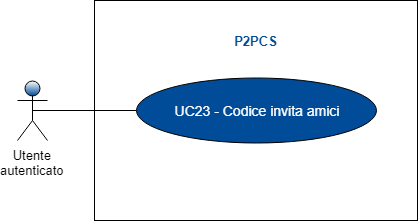
\includegraphics[width=9cm]{res/images/UC23Codiceamico.png}
	\centering
	\caption{UC26.2 - Estetica}
\end{figure}
\begin{itemize}
	\item \textbf{Attori Primari}: utente autenticato;
	\item \textbf{Descrizione}: l'utente accede alla categorie di modifiche sull'estetica per la propria auto. Avrà a disposizione un tot di materiale per ogni singola sottocategoria;
	\item \textbf{Scenario principale}: l'utente sta visualizzando la sua auto con una serie di modifiche da attuare per la categoria \textit{Estetica} quali:
	\begin{itemize}
		\item colore [UC26.2.1];
		\item adesivi [UC26.2.2];
		\item paraurti [UC26.2.3];
		\item fari [UC26.2.4];
		\item scarichi [UC26.2.5];
		\item cerchioni [UC26.2.6];
		\item alettoni [UC26.2.7].
	\end{itemize}
	\item \textbf{Precondizione}: L'utente ha intenzione di modificare la parte estetica della sua auto;
	\item \textbf{Postcondizione}: l'utente ha modificato gli elementi estetici della sua auto e potrà confermare l'installazione di tali modifiche.
\end{itemize}

\subsubsection{UC26.2.1 - Colore}
\begin{itemize}
	\item \textbf{Attori Primari}: utente autenticato;
	\item \textbf{Descrizione}: in questa sezione l'utente può modificare il motore della propria auto se in possesso di premi ricevuti da completamento di qualche obbiettivo o altro e di eventuali punti esperienza guadagnati col l'utilizzo continuo dell'applicazione.
	All'inizio viene messo a disposizione il modello base;
	\item \textbf{Scenario principale}: l'utente vuole modificare il motore della propria auto e verifica la presenza di motori migliori da poter installare, ma per pezzi non ancora sbloccati sarà possibile solo verificare i punti sulle statistiche oscurando l'immagine del pezzo stesso;
	\item \textbf{Precondizione}: l'utente ha scelto di modificare il motore del proprio veicolo; 
	\item \textbf{Postcondizione}: l'utente ha correttamente scelto un motore sbloccato da installare, in caso contrario terrà il modello base.
\end{itemize}
\subsubsection{UC26.1.2 - Centralina}
\begin{itemize}
	\item \textbf{Attori Primari}: utente autenticato;
	\item \textbf{Descrizione}: in questa sezione l'utente può modificare la centralina della propria auto se in possesso di premi ricevuti da completamento di qualche obbiettivo o altro e di eventuali punti esperienza guadagnati col l'utilizzo continuo dell'applicazione.
	All'inizio viene messo a disposizione il modello base;
	\item \textbf{Scenario principale}: l'utente vuole modificare la centralina della propria auto e verifica la presenza di centraline migliori da poter installare, ma per pezzi non ancora sbloccati sarà possibile solo verificare i punti sulle statistiche oscurando l'immagine del pezzo stesso;
	\item \textbf{Precondizione}: l'utente ha scelto di modificare la centralina del proprio veicolo; 
	\item \textbf{Postcondizione}: l'utente ha correttamente scelto una centralina sbloccata da installare, in caso contrario terrà il modello base.
\end{itemize}
\subsubsection{UC26.1.1 - Trasmissione}
\begin{itemize}
	\item \textbf{Attori Primari}: utente autenticato;
	\item \textbf{Descrizione}: in questa sezione l'utente può modificare la trasmissione della propria auto se in possesso di premi ricevuti da completamento di qualche obbiettivo o altro e di eventuali punti esperienza guadagnati col l'utilizzo continuo dell'applicazione.
	All'inizio viene messo a disposizione il modello base;
	\item \textbf{Scenario principale}: l'utente vuole modificare la trasmissione della propria auto e verifica la presenza di motori migliori da poter installare, ma per pezzi non ancora sbloccati sarà possibile solo verificare i punti sulle statistiche oscurando l'immagine del pezzo stesso;
	\item \textbf{Precondizione}: l'utente ha scelto di modificare la trasmissione del proprio veicolo; 
	\item \textbf{Postcondizione}: l'utente ha correttamente scelto una trasmissione sbloccata da installare, in caso contrario terrà il modello base.
\end{itemize}
\subsubsection{UC26.1.1 - Sospensioni}
\begin{itemize}
	\item \textbf{Attori Primari}: utente autenticato;
	\item \textbf{Descrizione}: in questa sezione l'utente può modificare le sospensioni della propria auto se in possesso di premi ricevuti da completamento di qualche obbiettivo o altro e di eventuali punti esperienza guadagnati col l'utilizzo continuo dell'applicazione.
	All'inizio viene messo a disposizione il modello base;
	\item \textbf{Scenario principale}: l'utente vuole modificare le sospensioni della propria auto e verifica la presenza di motori migliori da poter installare, ma per pezzi non ancora sbloccati sarà possibile solo verificare i punti sulle statistiche oscurando l'immagine del pezzo stesso;
	\item \textbf{Precondizione}: l'utente ha scelto di modificare le sospensioni del proprio veicolo; 
	\item \textbf{Postcondizione}: l'utente ha correttamente scelto le sospensioni sbloccate da installare, in caso contrario terrà il modello base.
\end{itemize}
\subsubsection{UC26.1.1 - Gomme}
\begin{itemize}
	\item \textbf{Attori Primari}: utente autenticato;
	\item \textbf{Descrizione}: in questa sezione l'utente può modificare le gomme della propria auto se in possesso di premi ricevuti da completamento di qualche obbiettivo o altro e di eventuali punti esperienza guadagnati col l'utilizzo continuo dell'applicazione.
	All'inizio viene messo a disposizione il modello base;
	\item \textbf{Scenario principale}: l'utente vuole modificare le gomme della propria auto e verifica la presenza di motori migliori da poter installare, ma per pezzi non ancora sbloccati sarà possibile solo verificare i punti sulle statistiche oscurando l'immagine del pezzo stesso;
	\item \textbf{Precondizione}: l'utente ha scelto di modificare le gomme del proprio veicolo; 
	\item \textbf{Postcondizione}: l'utente ha correttamente scelto le gomme sbloccate da installare, in caso contrario terrà il modello base.
\end{itemize} 
